\documentclass[a4paper,10pt]{article}
%\documentclass[a4paper,10pt]{scrartcl}

\usepackage[utf8]{inputenc}
%\usepackage{listings}
\usepackage{tikz}

\usetikzlibrary{arrows,automata}


\title{TP3 ACT}
\author{Matthieu Caron et Armand Bour}
\date{vendredi 9 octobre 2015}

\pdfinfo{%
  /Title    (TP2 ACT)
  /Author   (Matthieu Caron et Armand Bour)
  /Creator  (Matthieu Caron et Armand Bour)
  %/Producer ()
  %/Subject  ()
  %/Keywords ()
}

\begin{document}
\maketitle

\paragraph{Question 1}

Le code du graphique tikz est donné par Antoine Amara, mais la reflexion vient de nous 3.

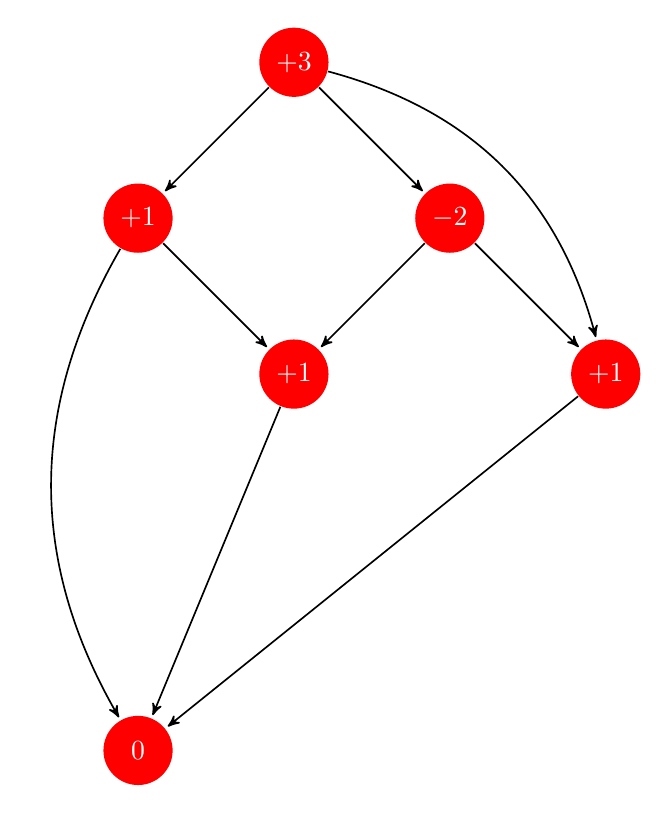
\begin{tikzpicture}[->,>=stealth',shorten >=1pt,auto,node distance=2.8cm,semithick]
    \tikzstyle{every state}=[fill=red,draw=none,text=white]
    \node[state] (A) {$+3$};
    \node[state] (B)[below left of=A] {$+1$};
    \node[state] (C)[below right of=A] {$-2$};
    \node[state] (D)[below left of=C] {$+1$};
    \node[state] (E)[below right of=C] {$+1$};
    \node[state] (F)[below of=D][below left of=E][below right of=B] {$0$};

    \path (A) edge              node {} (B)
    (B) edge                  node {} (D)
    (A) edge              node {} (C)
    (C) edge              node {} (D)
    (C) edge          node {} (E)
    (A) edge [bend left]         node {} (E)
    (B) edge [bend right]        node {} (F)
    (E) edge                     node {} (F)
    (D) edge                     node {} (F);
\end{tikzpicture}


\paragraph{Question 2}
S’ils sont tous positifs : $res = -1 * min(successeurs)-1$\newline
Sinon : $res = -1*max(desValeursNegatives) + 1$

\paragraph{Question 3}
La fonction récursive $naif$ calcule toutes les sous-tablettes possibles. Quatre boucles sont utilisées, une pour chaque possibilité de cassure (x colonne(s) à gauche ou à droite, et x ligne(s) en haut ou en bas). Des possibilités sont alors calculées plusieurs fois.\newline
En Python, la fonction prends en temps respectivement pour les configurations suivantes :
\begin{description}
\item[(10, 7, 7, 3)] 4 minutes 47 secondes ;
\item[(10, 7, 5, 3)] 10 minutes 24 secondes.
\end{description}

La différence de temps est due à la “profondeur” de la tête de mort dans la tablette. Dans le second cas, elle est plus proche du centre, ce qui décuple le nombre de sous-arbres possiblites.\newline
La complexité est exponentielle.

\paragraph{Question 4}
Notre algorithme est écrit en Python, et on ne sait pas pourquoi la version dynamique prend beaucoup de temps,
avec des print on a compté, l'initialisation du tableau pour dynamic(100,100,50,50) prend une dizaine de secondes.

\begin{description}
\item [(100, 100, 50, 50)] = -198.0
\item [(100, 100, 48, 52)] =

La version dynamique reste beaucoup plus rapide que la naive :
\begin{description}
\item[(10, 7, 7, 3)] en naïf prend 4 minutes 47 secondes ;
\item[(10, 7, 7, 3)] en dynamique prend 0,120 secondes.
\end{description}

\paragraph{Question 5}
Nous avons écrit la fonction pour déterminer les valeurs, mais étant donné la durée de l’algorithme, nous n’avons pas pu les obtenir.

\paragraph{Question 6}
Tout d’abord, on remplit le tableau qui dépend de $m$,$n$,$i$ et $j$ ce qui nous fait du $O(m*n*i*j)$
En suite dans l'algo on veut faire tous les découpages possible : ceux dans la largeur $m$, et ceux dans la longueur $n$.
Dans le calcul de la découpe, si le résultat a déjà été calculé, il s’agit simplemnet d’un accès au tableau, de complexité supposée en $O(1)$ (supposée car il n’y a aucune information concernant la complexité de l'objet utilisé $ndarray$ en Python). Sinon, il s’agit d’un calcul de toutes les sous-tablettes de chocolat.

\[
\left \{
\begin{array}{c}
    \mathsf{si\: deja\: calc\: alors}\: c(m,n) = 1 \\
    \mathsf{sinon} \sum_{k=1}^m c(m-k,n) + \sum_{l=1}^n c(m,n-l) 
\end{array}
\right.
\]

La complexité est alors en $O(m^2*n^2)$.

\paragraph{Question 7}
Toutes ces configurations ont la même valeur car il s’agit de la même plaque de chocolat soit pivotée d’un quart de tour, un demi-tour, trois quarts de tours, ou vue de dos (symétrique).

\paragraph{Question 8}
L'idée est d'ajouter quand c’est possible 8 valeurs au tableau plutôt qu'une seule (la valeur habituelle et les 7 autres configurations identiques).
En pratique, voici les tests effectués :
\begin{description}
\item[(30, 30, 10, 8)] en dynamique classique prend 3,91 secondes;
\item[(30, 30, 10, 8)] en dynamique avec symétrie prend 0,78 seconde.
\end{description}

\end{document}
